% Uncomment this to make slides with overlays:
%\documentclass[slides]{beamer}

% Uncomment these (but comment the above \documentclass line) to make handouts:
\documentclass[handout]{beamer}

% Uncomment these to have more than one slide per page
\usepackage{pgfpages}
\pgfpagesuselayout{2 on 1}[border shrink=5mm]
\pgfpageslogicalpageoptions{1}{border code=\pgfusepath{stroke}}
\pgfpageslogicalpageoptions{2}{border code=\pgfusepath{stroke}}

\usepackage[]{graphicx, color, hyperref}

\mode<presentation>
{
	%\usetheme[secheader]{Boadilla}
	%\usecolortheme[rgb={.835, .102,.169}]{structure}  
	\usetheme[width= 0cm]{Goettingen}
	%\setbeamercovered{transparent}
}
\setbeamertemplate{navigation symbols}{}
\setbeamertemplate{footline}[frame number]

\definecolor{blue2}{rgb}{0.278,0.278,0.729} 
\newcommand{\blue}[1]{\textcolor{blue2}{#1}}
\newcommand{\white}[1]{\textcolor{white}{#1}}
\newcommand{\red}[1]{\textcolor{red}{#1}}
\newcommand{\xbar}{\overline{x}}
\newcommand{\ybar}{\overline{y}}
\newcommand{\phat}{\widehat{p}}
\newcommand{\prob}{\mbox{Pr}}
\newcommand{\E}{\mathbb{E}}
\newcommand{\Var}{\mbox{Var}}
\newcommand{\cp}{\oplus}
\newcommand{\cm}{\circleddash}


\title{Lecture 17: Paired Data and Difference of Two Means}
\author{Chapter 5.2, 5.1}
\date{}


\begin{document}
%------------------------------------------------------------------------------
\begin{frame}
\titlepage
\end{frame}
%------------------------------------------------------------------------------


%------------------------------------------------------------------------------
\begin{frame}[fragile]
\frametitle{Goals for Today}

\begin{itemize}
\item Difference of means
\item Note on Practical vs Statistical Significance
\item Paired differences of means
\end{itemize}

\end{frame}
%------------------------------------------------------------------------------


%-------------------------------------------------------------------------------
\begin{frame}
\frametitle{6 Types of Questions}

Here are the 6 broad types of questions about \blue{population parameters} we'll be answering with statistical methods:  confidence intervals and hypothesis tests 

\vspace{0.25cm}

\begin{enumerate}
\pause\item What is the mean value $\mu$?
\pause\item Are the means $\mu_1$ and $\mu_2$ of two groups different?
\pause\item What is the mean paired difference $\mu_{diff}$?
\pause\item What is the proportion $p$ of ``successes''?
\pause\item Are the proportions of ``successes'' $p_1$ and $p_2$ of two groups different?
\pause\item Are the means $\mu_1, \ldots, \mu_k$ of $k$ groups different?
%\pause\item Are we observing counts that we were expected?
%\pause\item Are two categorical variables independent?
\end{enumerate}

\pause Today we look at 3 and 2.
\end{frame}
%-------------------------------------------------------------------------------


%------------------------------------------------------------------------------
\begin{frame}[fragile]
\frametitle{General Outline}
%We now generalize what we did in Chapter 4:
%\begin{enumerate}
%\pause\item Define the population parameter and determine its point estimate
%\pause\item Show that the sampling distribution of the point estimate is Normal
%\begin{itemize}
%\item Verify CLT \& any additional conditions
%\item Find the SE
%\end{itemize}
%\end{enumerate}
%
%\vspace{0.25cm}
%
%Then we either:
%\begin{itemize}
%\pause\item Build a confidence interval:  $\mbox{point estimate} \pm z^* SE$
%\pause\item Conduct a hypothesis test with test statistic:  $z$-score of the point estimate
%\[
%z=\frac{\mbox{point estimate} - \mbox{null value}}{SE}
%\]
%\end{itemize}

\end{frame}
%------------------------------------------------------------------------------


%total <- hist(run10Samp$time)
%F <- hist(run10Samp$time[run10Samp$gender=="F"])
%M <- hist(run10Samp$time[run10Samp$gender=="M"])
%
%mean.m <- mean(run10Samp$time[run10Samp$gender=="M"])
%mean.f <- mean(run10Samp$time[run10Samp$gender=="F"])
%
%pdf("./7.3 Paired Data + Diff of Two Mean/race.pdf", width=6, height=6)
%hist(run10Samp$time[run10Samp$gender=="M"], breaks=total$breaks, col='cyan',
%     border='cyan', xlab="Race Time (in minutes)", main="Cherry Blossom Run Times", 
%     ylim=c(0,max(F$counts, M$counts)))
%hist(run10Samp$time[run10Samp$gender=="F"],add=T)
%legend("topright", 
%       legend=c("men", "women"), 
%       fill=c("cyan", "white"),
%       bty='n')
%dev.off()
%------------------------------------------------------------------------------
\begin{frame}[fragile]
\frametitle{Chapter 5.2: Are Two Means $\mu_1$ \& $\mu_2$ Different?}

We randomly sample 45 men (of 7192) and 55 women (of 9732) runners in the 2012 Cherry Blossom Run. \pause \blue{Did men run faster than women?}

\begin{columns}
%--------------------------
\pause\column{.6\textwidth}
\begin{center}
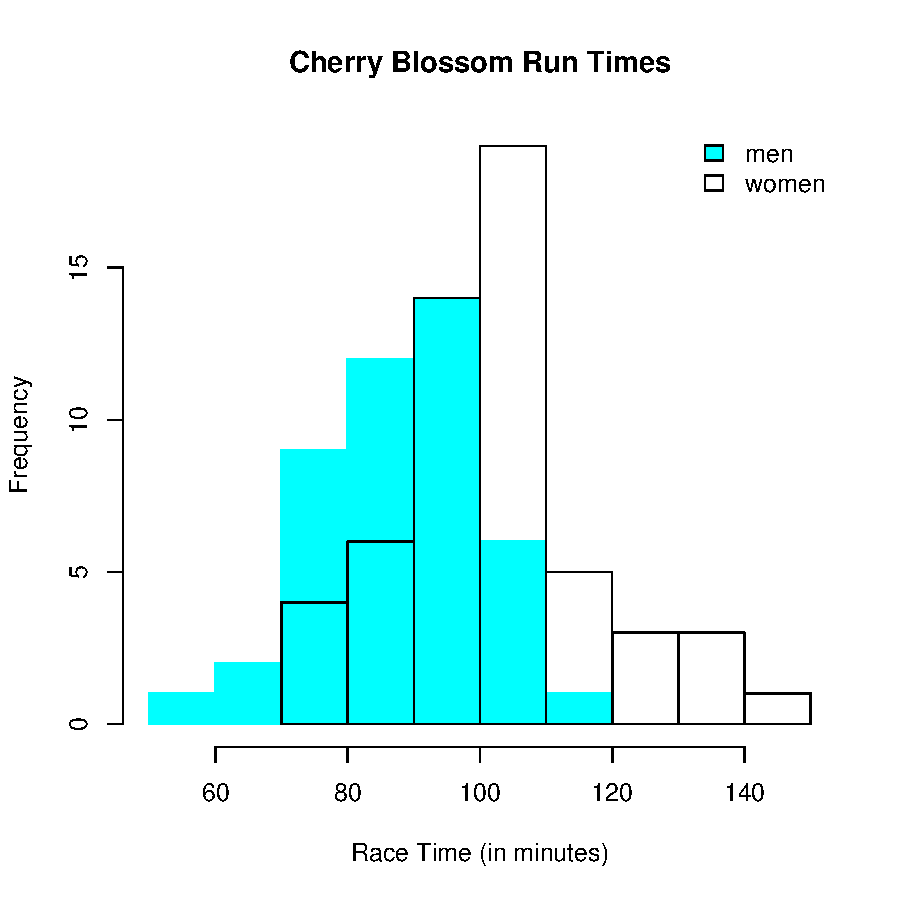
\includegraphics[width=\textwidth]{figure/race.pdf}
\end{center}
%--------------------------
\pause\column{.3\textwidth}
\begin{center}
\begin{tabular}{c|rr}
     & men & women \\ 
\hline
    $\overline{x}$ & 87.65 & 102.13 \\ 
    $s$ & 12.5 & 15.2 \\ 
    $n$ & 45 & 55 \\ 
\end{tabular}
\end{center}
%--------------------------
\end{columns}

\end{frame}
%------------------------------------------------------------------------------


%------------------------------------------------------------------------------
\begin{frame}[fragile]
\frametitle{Difference in Means}
%We want the difference of two population means:
%\pause\begin{itemize}
%\item $\mu_w$: mean time for women
%\item $\mu_m$: mean time for men
%\end{itemize}
%
%Thus:
%\begin{itemize}
%\pause\item Population parameter:  $\mu_w - \mu_m$.\\
%i.e. if men run faster, this is positive
%\pause\item Point estimate:  $\xbar_w - \xbar_m = 102.13-87.65=14.48$\\
%i.e. \blue{difference of sample means}
%\end{itemize}
\end{frame}
%------------------------------------------------------------------------------


%------------------------------------------------------------------------------
\begin{frame}[fragile]
\frametitle{Normality of Sampling Distribution}
%If two sample means $\xbar_1$ and $\xbar_2$ 
%\begin{itemize}
%\pause\item each satisfy the 3 CLT conditions
%\pause\item Additionally: the \blue{two samples are independent from each other}
%\end{itemize}
%
%\vspace{0.25cm}
%
%\pause Then the sampling distribution of $\xbar_1 - \xbar_2$ will be approximately normal with
%\begin{itemize}
%\pause\item mean $\mu_1-\mu_2$
%\pause\item estimated standard error
%\[
%SE_{\xbar_1 - \xbar_2} = \sqrt{\frac{\sigma_1^2}{n_1} + \frac{\sigma_2^2}{n_2}} \approx \sqrt{\frac{s_1^2}{n_1} + \frac{s_2^2}{n_2}}
%\]
%\end{itemize}
\end{frame}
%------------------------------------------------------------------------------


%------------------------------------------------------------------------------
\begin{frame}[fragile]
\frametitle{Normality of Sampling Distribution}
%We verify the conditions:
%\begin{enumerate}
%\pause\item Each sample consists of $\leq$10\% of their respective populations.
%\pause\item Both histograms don't look too skewed.
%\pause\item Each sample has at least 30 observations (rule of thumb).
%\pause\item \blue{Additionally}: the samples are independent (not paired or linked in any way).
%\end{enumerate}
%
%\pause\vspace{0.25cm}
%
%Thus the sampling distribution is Normal with mean=$\mu_w - \mu_m$ and
%\[
%SE_{\xbar_w - \xbar_m} = \sqrt{\frac{15.2^2}{55} + \frac{12.5^2}{45}} = 2.77
%\]
\end{frame}
%------------------------------------------------------------------------------


%------------------------------------------------------------------------------
\begin{frame}[fragile]
\frametitle{Confidence Interval}
%A 95\% confidence interval for $\mu_1 - \mu_2$ is
%\begin{eqnarray*}
%(\mbox{point estimate for } \mu_1 - \mu_2) &\pm& z^* \times SE\\
%\pause(\xbar_1 - \xbar_2) &\pm& 1.96 \times SE_{\xbar_1 - \xbar_2}
%\end{eqnarray*}
%
%\pause\vspace{0.25cm}
%
%\pause For the Cherry Blossom Run data, a 95\% CI for $\mu_w - \mu_m$ is:
%\begin{eqnarray*}
%14.48 \pm 1.96 \times 2.77 =  [9.05, 19.91]
%\end{eqnarray*}
\end{frame}
%------------------------------------------------------------------------------


%------------------------------------------------------------------------------
\begin{frame}[fragile]
\frametitle{Hypothesis Test}
%For $\alpha=0.001$ (i.e. we want reject with high confidence) we test
%\begin{itemize}
%\item $H_0: \mu_w - \mu_m = 0$
%\item $H_A: \mu_w - \mu_m > 0$
%\end{itemize}
%
%\pause\vspace{0.25cm}
%
%Test statistic:  $z$-score of $\xbar_w - \xbar_m$ under $H_0$:
%\begin{eqnarray*}
%\frac{\mbox{point estimate} - \mbox{null value}}{SE} &=& \frac{(\xbar_w - \xbar_m) - \mbox{null value}}{SE_{\xbar_1 - \xbar_2}}\\
%&=& \frac{14.48 - 0}{2.77} = 5.23
%\end{eqnarray*}
%
%\pause\vspace{0.25cm}
%
%The p-value is $0$, hence we reject $H_0$ and declare that men ran significantly faster than women.  

\end{frame}
%------------------------------------------------------------------------------


%------------------------------------------------------------------------------
\begin{frame}
\frametitle{Practical vs Statistical Significance}
When rejecting $H_0$, we call this a \blue{statistically significant} result.  But statistically significant results aren't always \blue{practically significant}.

\pause\vspace{0.5cm}

Say for \blue{very} large $n_M$ \& $n_F$ we observe $\xbar_M = 87.65$ and $\xbar_F = 87.651$ and reject $H_0$.  

\pause\vspace{0.5cm}

The point estimate of the difference $\xbar_M - \xbar_F = 0.001$.  Near negligible!  

\pause\vspace{0.5cm}

However, the 95\% CI might be:
\[
[0.0005, 0.0015]
\]

\end{frame}
%------------------------------------------------------------------------------


%------------------------------------------------------------------------------
\begin{frame}
\frametitle{Practical vs Statistical Significance}

Moral of the story

\begin{itemize}
\pause\item Hypothesis tests with ``rejections of $H_0$'' focus almost entirely on \blue{statistical significance}.
\pause\item Confidence intervals allow you to also focus on \blue{practical significance}.  
\end{itemize}

\end{frame}
%------------------------------------------------------------------------------


%------------------------------------------------------------------------------
\begin{frame}[fragile]
\frametitle{Chapter 5.1: Paired Data}
Two sets of observations are \blue{paired} if each observation in one set has a special correspondence or connection with exactly one observation in the other data set.

\vspace{0.25cm} 

\pause Examples:

\begin{itemize}
\item Cholesterol levels before and after some intervention for the same person
\pause \item Disease rates amongst pairs of twins
\pause \item In the text:  price of the same textbook at the UCLA bookstore vs Amazon
\end{itemize}

\end{frame}
%------------------------------------------------------------------------------


%pdf("./7.3 Paired Data + Diff of Two Mean/diff.pdf", width=7, height=5)
%plot(textbooks$uclaNew, pch=19, log='y', xlab="Textbook #", ylab="Price",
%     main="UCLA & Amazon Price for Each Textbook")
%points(textbooks$amazNew, pch=19, col="red")
%legend("topleft", legend=c("UCLA","Amazon"), pch=c(19,19), col=c(1,2))
%dev.off()
%
%pdf("./7.3 Paired Data + Diff of Two Mean/diff2.pdf", width=7, height=5)
%plot(textbooks$uclaNew - textbooks$amazNew, pch=19, 
%     xlab="Textbook #", ylab="Difference in Price",
%     main="UCLA Price - Amazon Price")
%abline(h=0)
%dev.off()
%
%pdf("./7.3 Paired Data + Diff of Two Mean/diff2.pdf", width=7, height=5)
%boxplot(textbooks$uclaNew - textbooks$amazNew, horizontal=TRUE, xlab="UCLA Price - Amazon Price")
%dev.off
%------------------------------------------------------------------------------
\begin{frame}[fragile]
\frametitle{Paired Differences}
The methodology for paired data remains the same, except our \blue{observations} are the difference in pairs.  Example, for the UCLA Bookstore vs Amazon book price example in the text
\begin{center}
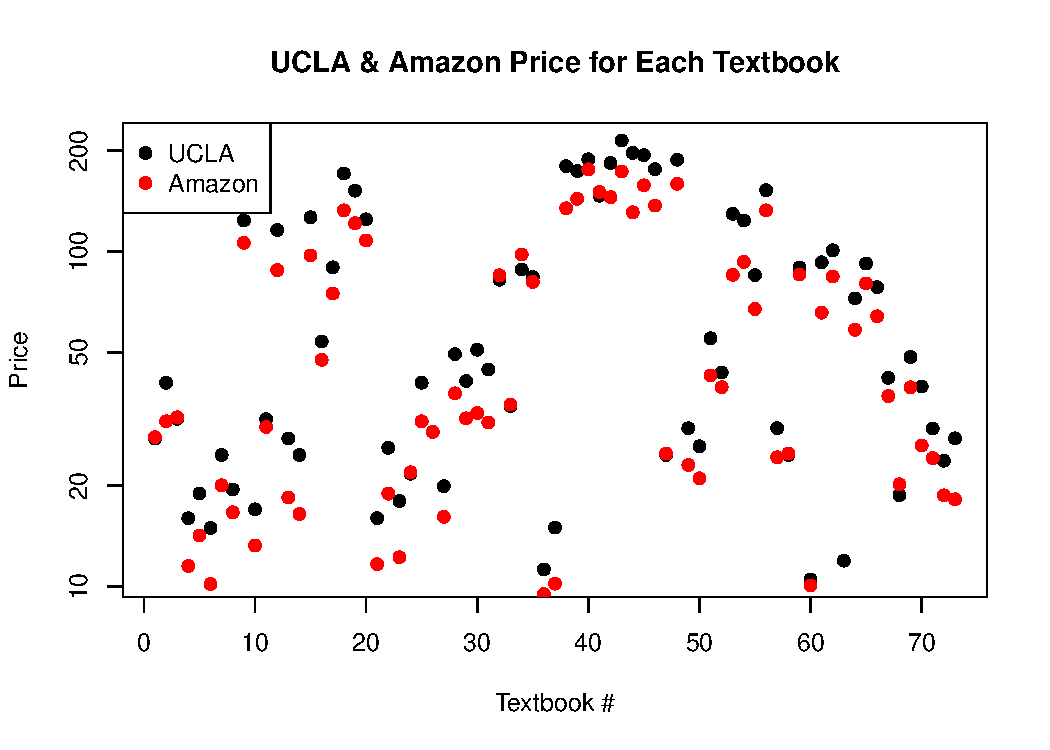
\includegraphics[width=0.8\textwidth]{figure/diff.pdf}
\end{center}


\end{frame}
%------------------------------------------------------------------------------


%------------------------------------------------------------------------------
\begin{frame}[fragile]
\frametitle{Paired Differences}
The methodology for paired data remains the same, except our \blue{observations} are the difference in pairs.  Example, for the UCLA Bookstore vs Amazon book price example in the text
\begin{center}
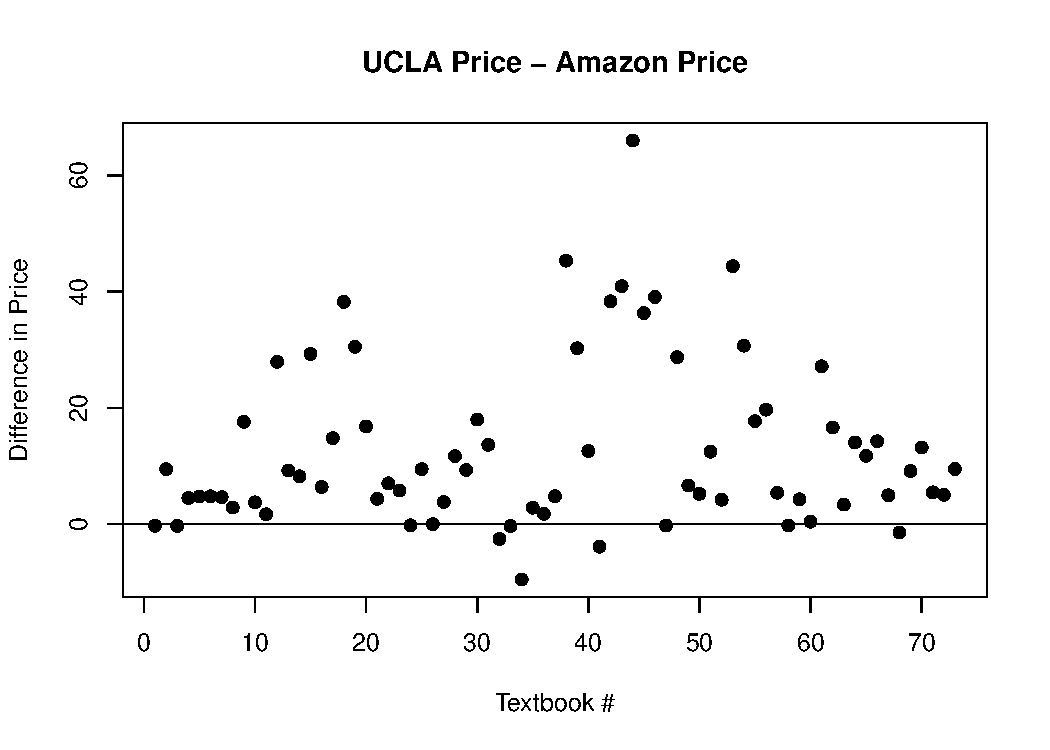
\includegraphics[width=0.8\textwidth]{figure/diff2.pdf}
\end{center}


\end{frame}
%------------------------------------------------------------------------------


%------------------------------------------------------------------------------
\begin{frame}[fragile]
\frametitle{Paired Differences}
We have
\begin{itemize}
\pause \item population parameter is $\mu_{diff}$ with point estimate $\xbar_{diff}$
\pause \item Check the conditions not on the original observations, but rather the \blue{differences}.
\pause \item If met, $\xbar_{diff}$ has a normal sampling distribution
\begin{itemize}
\item mean $\mu_{diff}$
\item $SE_{diff} = \frac{\sigma_{diff}}{\sqrt{n_{diff}}} \approx \frac{s_{diff}}{\sqrt{n_{diff}}}$
\end{itemize} 
\end{itemize}


\end{frame}
%------------------------------------------------------------------------------


%------------------------------------------------------------------------------
\begin{frame}[fragile]
\frametitle{Next Time}

\begin{itemize}
\item t-test
\end{itemize}


\end{frame}
%------------------------------------------------------------------------------


\end{document}





